\section{Modulare Views}
\label{mv-main}

Modularen Views sind \glspl{ui}, die aus wiederverwendbaren Komponenten bestehen. Diese Komponenten sind gekapselt und können dadurch an unterschiedlichen Stellen in eine Anwendung eingebunden werden. Durch dieses Prinzip erhöht sich die Wartbarkeit und Testbarkeit der Anwendung, da die einzelnen Komponenten isoliert voneinander existieren. Einzelne Komponenten erfüllen dabei den Grundsatz \glqq Don't-Repeat-Yourself\grqq{}. Ein Konzept, das dieses Prinzip für Webtechnologien umsetzt, nennt sich WebComponents. WebComponents sind wiederverwendbare \gls{ui}-Komponenten, die mit Webtechnologien erstellt werden. WebComponents bestehen aus vier separaten Standards, die gemeinsam oder einzeln genutzt werden können \cite{WebComponentsStandards}. Mittels WebComponents lassen sich demnach eigene HTML-Elemente definieren und nutzen. In diesen Elementen können \gls{css} und JavaScript verwendet werden, ohne dass dies einen Einfluss auf die äußere Anwendung hat \cite{WebComponents}. Leider sind WebComponents derzeit noch in der Entwicklungsphase und werden nicht vollständig von allen gängigen Browsern unterstützt \cite{WebComponentsVerfuegbarkeit}. AngularJS stellt jedoch Features bereit, die denen der WebComponents sehr ähnlich sind. Über AngularJS Direktiven lassen sich ebenfalls eigene \gls{html}-Elemente sowie Attribute definieren. Neben Direktiven gibt es jedoch noch eine weitere Möglichkeit, externe \gls{html}-Fragmente in eine Datei einzubinden. Doch welche Methode ist hinsichtlich der Performance besser? Dieser Frage soll hier nachgegangen werden. Zunächst wird dazu der Kompilier- und Link-Prozess von AngularJS betrachtet, der diese Verfahren erst ermöglicht. Anschließend werden basierend darauf, die beiden Möglichkeiten untersucht und im Anschluss mittels Zeitmessungen verglichen. 

\subsection{AngularJS Kompilier- und Link-Phase}
\label{angularjskompilierundlinkphase}
AngularJS ermöglicht über Direktiven das Erstellen von selbst definierten \gls{html}-Elementen und Attributen. Da sich WebComponents zurzeit noch in der Entwicklung befinden, implementiert AngularJS diese Technik auf eine andere Art und Weise. Zunächst werden Direktiven über AngularJS definiert. Diese Direktiven können anschließend im \gls{html} platziert werden. Beim Anzeigen einer Seite führt AngularJS einen Kompiliervorgang durch. Dieser Prozess besteht aus der Compile-Phase und der Link-Phase. In der Compile-Phase wird der gesamte \gls{dom} durchlaufen und hinsichtlich der Verwendung von Direktiven geprüft. Jede verwendete Direktive kann eine eigene \emph{compile}-Methode besitzen, die in dieser Phase ausgeführt wird. Darin können Modifikationen am \gls{dom} durchgeführt werden. Die \emph{compile}-Methode wird dabei nur einmalig ausgeführt, auch wenn die Direktive mehrfach verwendet wird. In der Link-Phase verknüpft die \emph{link}-Methode die Instanz einer Direktive mit einem Model (\emph{\$scope}). Darin können \gls{DOMListener} oder Two-Way-Databindings initialisiert werden.\cite{AJSCompileAndLink}
\\\\
Selbst erstellten Direktiven kann ein \gls{html}-Template, sowie ein eigener Controller zugewiesen werden. Zusätzlich erhält jede Direktive in der Link-Phase ein Model. Bei der Definition der Direktive legt man fest, ob dies ein neues Model, oder ein bereits im \gls{dom} befindliches übergeordnetes Model sein soll. Letzteres ermöglicht den Zugriff auf Eigenschaften in der äußeren Anwendung. Der Nachteil ist jedoch die dadurch fehlende Kapselung der Komponente, was sich negativ auf die Wartbarkeit auswirkt. Stattdessen können bei einem neuen Model über Parameter Werte von der äußeren Anwendung an die Direktive übergeben werden.\cite{AJSDirectives}

\subsection{Direktive ngInclude}
AngularJS enthält bereits eine Vielzahl fertiger Direktiven. Die Direktive \emph{ngInclude} wird dazu verwendet, ein externes \gls{html}-Fragment in ein Dokument einzubinden. Es kann dafür als \gls{html}-Element oder Attribut angewendet werden und benötigt lediglich den Pfad zur Datei als Parameter. In der Kompilier-Phase von AngularJS wird diese Direktive durch das angegebene \gls{html}-Fragment ersetzt. Dabei wird zunächst das Dokument über die Netzwerkschnittstelle geladen, anschließend selbst kompiliert und danach in den \gls{dom} eingefügt. Das Kompilieren ist notwendig, da sich in diesem \gls{html}-Fragment wiederum AngularJS spezifische Inhalte befinden können. 
\begin{lstlisting}[language=HTML,style=ionicHtmlStyle,caption={Modulare Views, Verwendung von ngInclude}\label{mv-nginclude}]
<!-- book.html -->
<img ng-src="{{::book.image}}"></img>
<h2>{{::book.name}}</h2>
<h3>{{::book.author}}</h3>
<p>{{::book.description}}</p>
<p>{{::book.price}}</p>

<!-- Verwendung -->
<ion-list>
	<ion-item ng-repeat="book in books">
		<div ng-include="'.../book.html'"></div>
	</ion-item>
</ion-list>
\end{lstlisting}
Der Nachteil von \emph{ngInclude} im Vergleich zu einer Direktive ist die fehlende Flexibilität und Kapselung. Dem eingebundenen Fragment wird kein eigenes Model zugewiesen. Es hat direkten Zugriff auf Eigenschaften in der äußeren Anwendung. Ein weiterer Nachteil ist der eigene Kompiliervorgang. Wird ein Fragment über diesen Mechanismus mehrfach auf einer Seite eingefügt, wird bei jeder Instanz die Compile-Phase durchgeführt. Bei einer Direktive hingegen nur einmalig. Dies wirkt sich vor allem bei Listen auf das Antwortzeitverhalten aus. Listing \ref{mv-nginclude} zeigt die Verwendung von \emph{ngInclude} in einer Liste als \gls{html}-Attribut. Die Datei \emph{book.html} verwendet dabei die Variable \emph{book}, obwohl sie im Kontext dieser Datei nicht auftaucht. Erst in Kombination mit der Verwendung erfüllt dieses \gls{html}-Fragment einen Zweck. Das unterstreicht noch einmal die fehlende Kapselung. Der Vorteil von \emph{ngInclude} ist die simple Verwendung. Es ist keine zusätzliche Definition erforderlich und bietet sich dadurch an, um komplexe Views zu separieren, ohne dass die einzelnen Teile eine eigene Logik enthalten.\cite{AJSNGInclude}

\subsection{Benutzerdefinierte Direktiven}
Um \gls{ui}-Komponenten in AngularJS zu erstellen sind Direktiven eine sinnvolle Möglichkeit. Sie bieten die größtmögliche Flexibilität im Hinblick auf die Verwendung der Komponente. So können Direktiven als \gls{html}-Element, \gls{html}-Attribut oder sogar als \gls{css}-Klasse eingebunden werden. Zusätzlich kann die Komponente über ein \gls{Template} Inhalte präsentieren, durch einen Controller eine eigene Logik implementieren und über entsprechende Methoden den \gls{dom} manipulieren. Darüber hinaus kann eine Direktive als Container eingesetzt werden, um Inhalte in sich zu vereinen. Über eine Konfiguration wird der Direktive ein eigenes Model zugewiesen (Kapselung). Alternativ hat sie ähnlich wie \emph{ngInclude} direkten Zugriff auf die äußere Anwendung. Die konkrete Funktionsweise einer Direktive wurde bereits in Abschnitt \ref{angularjskompilierundlinkphase} beschrieben. Die Vor- und Nachteile ergeben sich entgegengesetzt den Vor- und Nachteilen von \emph{ngInclude}. 
\begin{lstlisting}[language=JavaScript, caption={Modulare Views, Definition einer Direktive}\label{mv-directive-definition}]
var app = angular.module('ba');
app.directive('book', function() {
	return {
		restrict: 'E', // E = Element -> DOM-Element (A = Attribute)
		scope: {
			mybook: '=book'
		},
		templateUrl: '.../book.html'
	}
});
\end{lstlisting}
Listing \ref{mv-directive-definition} zeigt die Definition einer Direktive, die als \gls{html}-Element verwendet werden kann und ein \gls{Template} sowie ein isoliertes Model besitzt. Durch die Angabe der Eigenschaft \emph{scope} kann die Direktive nicht auf Eigenschaften der äußeren Anwendung zugreifen, sondern nur auf die in diesem Fall selbst definierte Eigenschaft \emph{mybook}. Die Verwendung in Listing \ref{mv-directive-usage} macht deutlich, dass Direktiven eine intuitive Anwendung ermöglichen. Über die Parameter der Direktive und das isolierte Model existiert eine klare Schnittstelle. 
\begin{lstlisting}[language=HTML,style=ionicHtmlStyle,caption={Modulare Views, Verwendung einer Direktive}\label{mv-directive-usage}]
<!-- book.html -->
<img ng-src="{{::mybook.image}}"></img>
<h2>{{::mybook.name}}</h2>
<h3>{{::mybook.author}}</h3>
<p>{{::mybook.description}}</p>
<p>{{::mybook.price}}</p>

<!-- Verwendung -->
<ion-list>
	<ion-item ng-repeat="book in books">
		<book mybook="book"></book>
	</ion-item>
</ion-list>
\end{lstlisting}
		
\subsection{Analyse des Optimierungspotentials}
In diesem Abschnitt werden beide Varianten hinsichtlich ihrer Performance untersucht. Relevant dabei ist die Zeit, die für das Einfügen der jeweiligen Komponente in eine View benötigt wird. Diese Zeit beeinflusst maßgeblich das Antwortzeitverhalten der App bei Seitenübergängen. 
\begin{figure}[h]
	\centering
	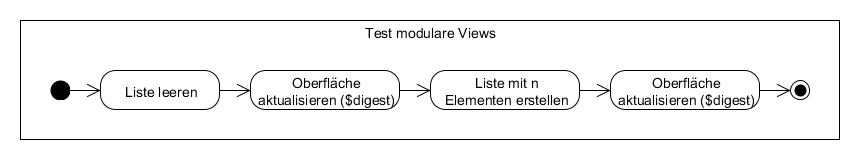
\includegraphics[scale=0.4]{Bilder/Testablauf-ModularView.png}
	\caption{Testablauf für das Einfügen modulare Komponenten in eine View}
	\label{test-modulareview}
\end{figure}
Für diesen Test werden in der Testanwendung zwei Module angelegt. Dabei entsteht jeweils eine Seite mit Tests für Direktiven und eine für \emph{ngInclude}. Die Vorgehensweise des Tests wird durch Abbildung \ref{test-modulareview} verdeutlicht. Getestet wird jeweils das Einfügen von \emph{n} Elementen in eine Liste. Die Anzahl kann in der Oberfläche frei konfiguriert werden. Um bei jedem Zyklus von BenchmarkJS gleiche Bedingungen zu schaffen, wird die Liste vor jedem Durchlauf geleert. Nach dem Leeren und neu Befüllen werden die Änderungen jeweils durch einen \emph{\$digest}-Zyklus in die View übertragen. Ein asynchroner Timer sorgt jeweils dafür, dass Render- und Layout-Prozesse abgeschlossen sind, bevor der Test weitergeführt wird. In JavaScript wird dazu häufig ein Timer mit der Dauer 0 eingesetzt. Dieser Timer erhält eine JavaScript-Funktion, welche ausgeführt wird, sobald alle anderen Aufgaben der Browser-Engine abgeschlossen sind. 
\\\\
Durch diesen Test wird die Zeit für den gesamten Prozess gemessen und nicht nur das reine Einfügen der Elemente in die Liste. Das Ergebnis gibt somit keine Auskunft über die konkrete Laufzeit des Einfügens. Stattdessen zeigen die Ergebnisse das Verhältnis zwischen den Zeitmessungen beider Varianten und ermöglichen einen direkten Vergleich. Das Ergebnis in Abbildung \ref{mv-benchjs-analyse} zeigt deutlich, dass Direktiven beim Einfügen in eine View unter Android 4.4.4 im Mittel 26\% schneller sind als \emph{ngInclude}. Die Erwartung, dass die Zeiten bei einem einzigen Element etwa gleich sind, ist nicht eingetroffen. Selbst dabei ist eine deutliche Steigerung sichtbar, obwohl die Compile- und Link-Phase gleichermaßen angewendet wird. Eine Direktive wird nur ein einziges mal kompiliert, unabhängig davon, wie oft sie in einer App verwendet wird. Das \gls{html}-Fragment bei \emph{ngInclude} wird hingegen bei jedem Einbinden kompiliert. Dieser Unterschied spiegelt sich in diesen Ergebnissen nicht wider. 
\\\\
Neben den Vorteilen durch die Kapselung und die größere Flexibilität sollte eine Direktive demnach immer vorgezogen werden, sobald mehr als eine Element in einer Oberfläche eingefügt werden soll. \emph{ngInclude} eignet sich dadurch lediglich für die Verringerung der Komplexität eines Templates in großen \glspl{ui}.
\\\\
Eine weitere teils erstaunliche Beobachtung der Ergebnisse zeigt, dass die Laufzeiten unter Android 4.3 im Mittel 32\% schneller sind als unter Android 4.4.4. Dies deckt sich nicht mit der zu Anfang erwähnten Performancesteigerung durch die neue Browser-Engine.
\begin{figure}[h]
	\centering
	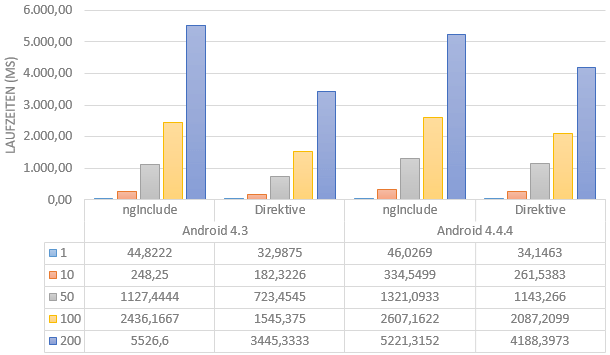
\includegraphics[scale=0.9]{Bilder/Diagramme/ModulareViews.png}
	\caption{Modulare Views - Laufzeitmessung ngInclude vs. Direktive}
	\label{mv-benchjs-analyse}
\end{figure}